\documentclass[symmetric,justified,marginals=justified,notoc]{tufte-book}

%-------------
% PACKAGES
%-------------
\usepackage{lipsum,graphicx,amsfonts,amsmath,amsthm,xcolor,ifthen,epstopdf}
\usepackage[shortlabels]{enumitem}
\usepackage[strict]{changepage}
\usepackage{mdframed}

\usepackage{ouractivities}

%--------------
% COMMANDS
%--------------
\newcounter{cnt}
\newenvironment{numlist}{\begin{list}{(\arabic{cnt})}{\usecounter{cnt}
\setlength{\leftmargin}{.35 in}\setlength{\labelwidth}{.35 in}
\setlength{\itemsep}{10 pt}}}{\end{list}}

\newcounter{cnt4}
\newenvironment{numlist2}{\begin{list}{(\arabic{cnt4})}{\usecounter{cnt4}
\setlength{\leftmargin}{.5 in}\setlength{\labelwidth}{.25 in}
\setlength{\itemsep}{10 pt}}}{\end{list}}

\newcounter{cnt2}
\newenvironment{alphalist}{\vspace*{-3 pt}\begin{list}{(\alph{cnt2})}{\usecounter{cnt2}
\setlength{\leftmargin}{.5 in}\setlength{\labelwidth}{.25
in}\setlength{\itemsep}{5 pt}}}{\end{list}}

\newcounter{cnt3}
\newenvironment{alphalist2}{\vspace*{-3 pt}\begin{list}{(\alph{cnt3})}{\usecounter{cnt3}
\setlength{\leftmargin}{.25 in}\setlength{\labelwidth}{.25
in}\setlength{\itemsep}{5 pt}}}{\end{list}}

\newcounter{cnt5}
\newenvironment{thmlist}{\vspace*{-3 pt}\begin{list}{{\em (\roman{cnt5})}}{\usecounter{cnt5}
\setlength{\leftmargin}{.5 in}\setlength{\labelwidth}{.25
in}\setlength{\itemsep}{3 pt}}}{\end{list}}

\newcommand{\be}{\begin{numlist}}
\newcommand{\ee}{\end{numlist}}
\newcommand{\bei}{\begin{numlist2}}
\newcommand{\eei}{\end{numlist2}}
\newcommand{\bal}{\begin{alphalist2}}
\newcommand{\eal}{\end{alphalist2}}
\newcommand{\bi}{\begin{itemize}}
\newcommand{\ei}{\end{itemize}}
\newcommand{\btl}{\begin{thmlist}}
\newcommand{\etl}{\end{thmlist}}

% theorem-like environments
\theoremstyle{definition}
%\newtheorem{pa}{Preview Activity}[chapter]
%\newtheorem{example}{Example}[chapter]
%\newtheorem{definition}{Definition}[chapter]

%\newcommand{\bex}{\begin{center}\underline{\hspace{5.0in}}\end{center} \begin{example}}
%\newcommand{\eex}{ \noindent{\bf Solution.}~~}

\newcommand{\afterexercises}{\nin \hrulefill \vfill \ \newpage}

% my commands

\newcommand{\ds}{\ensuremath{\displaystyle}}
\newcommand{\nin}{\noindent}
\newcommand{\tr}{\vspace*{0.5in}}
\newcommand{\lr}{\vspace*{1.0in}}
\newcommand{\mr}{\vspace*{2.0in}}
\newcommand{\br}{\vspace*{3.0in}}


\newcommand\T{\rule{0pt}{2.6ex}}
\newcommand\B{\rule[-1.2ex]{0pt}{0pt}}

\newcommand{\vs}{\vspace*{0.1in}}
\newcommand{\solution}{\noindent{\bf Solution.}}
%--------------------
% END COMMANDS
%--------------------

%---------------------
% BEGIN DOCUMENT
%---------------------
\begin{document}

\begin{goals}
\item How is the average velocity of a moving object connected to the values of its position function?
\item How do we interpret the average velocity of an object geometrically with regard to the graph of its position function?
\item How is the notion of instantaneous velocity connected to average velocity?
\end{goals}

\begin{marginfigure}[8cm]
\margingraphics{figures/1_2_PA1.eps} 
\caption{Graph of $y = g(x)$ for Preview Activity~\ref{PA:1.1}.} \label{fig:1.1.PA1}
\end{marginfigure}

\begin{pa} \label{PA:1.1}
Suppose that $g$ is the function given by the Figure~\ref{fig:1.1.PA1}.  Use the graph to answer each of the following questions. 
\ba
	\item Determine the values $g(-2)$, $g(-1)$, $g(0)$, $g(1)$, and $g(2)$, if defined.  If the function value is not defined, explain what feature of the graph tells you this.
	\item For each of the values $a = -1$, $a = 0$, and $a = 2$, complete the following sentence: ``As $x$ gets closer and closer (but not equal) to $a$, $g(x)$ gets as close as we want to \underline{\hspace{0.3in}}.''
	\item What happens as $x$ gets closer and closer (but not equal) to $a = 1$?  Does the function $g(x)$ get as close as we would like to a single value?
\ea

\end{pa} \afterpa

\begin{margintable}[6cm]
\begin{tabular}{c|c||c|c}
	$x$ & $f(x)$ & $x$ & $f(x)$ \\ \hline
	$0.5$ & $1.5$ & $1.5$ & \hspace{.75in} \\
	$0.9$ & \hspace{.75in} & $1.1$ & $2.1$ \\
	$0.99$ & $1.99$ & $1.01$ & \hspace{.75in} \\
	$0.999$ & \hspace{.75in} & $1.001$ & $2.001$ \\
\end{tabular}
\caption{Tabe of values near $x=1$.}
\label{T:1-1_Act1}
\end{margintable}

\begin{activity} \label{A:1.1.1}  Consider the function $f(x) = \dfrac{x^2 - 1}{x - 1}$.
\ba
\item Does the value of $f(1)$ exist? Why/why not?

\item Use a calculator or spreadsheet to fill in the blanks of Table~\ref{T:1-1_Act1}. Some of these have already been done for you; your calculations should not be drastically different from the ones already here. For example a calculation equal to 22.5 is very likely incorrect. Based on the table, estimate the value of $\ds \lim_{x \to 1} \frac{x^2 - 1}{x-1}$. 

\item Plot an accurate graph of the function $f$.  It should be a straight line.  Using your plot, what is $f(1)$?  What is $\ds \lim_{x \to 1} f(x)$?

\item Now use algebra to simplify the fraction $\dfrac{x^2 - 1}{x - 1}$. Call this new function $g(x)$.  What is $\ds \lim_{x \to 1} g(x)$? How is this limit related to the limit of $f(x)$ as $x$ approaches $1$?
\ea
\end{activity}

\aftera


\bex
For a falling ball whose position function is given by $s(t) = 16 - 16t^2$ (where $s$ is measured in feet and $t$ in seconds), find an expression for the average velocity of the ball on a time interval of the form $[0.5, 0.5+h]$ where $-0.5 < h < 0.5$ and $h \ne 0$.  Use this expression to compute the average velocity on $[0.5,0.75]$ and $[0.4,0.5]$, as well as to make a conjecture about the instantaneous velocity at $t = 0.5$.
\eex
We make the assumptions that $-0.5 < h < 0.5$ and $h \ne 0$ because $h$ cannot be zero (otherwise there is no interval on which to compute average velocity) and because the function only makes sense on the time interval $0 \le t \le 1$, as this is the duration of time during which the ball is falling.  Observe that we want to compute and simplify $$AV_{[0.5, 0.5+h]} = \frac{s(0.5+h) - s(0.5)}{(0.5+h) - 0.5}.$$  The most unusual part of this computation is finding $s(0.5+h)$.  To do so, we follow the rule that defines the function $s$.  In particular, since $s(t) = 16-16t^2$, we see that \begin{eqnarray*}
  s(0.5+h) & = & 16 - 16(0.5 + h)^2 \\
  		& = & 16 - 16(0.25 + h + h^2) \\
		& = & 16 - 4 - 16h - 16h^2 \\
		& = & 12 - 16h - 16h^2.
\end{eqnarray*}
Now, returning to our computation of the average velocity, we find that 
\begin{eqnarray*}
 AV_{[0.5, 0.5+h]} & = & \frac{s(0.5+h) - s(0.5)}{(0.5+h) - 0.5} \\
 			& = & \frac{(12 - 16h - 16h^2) - (16 - 16(0.5)^2)}{0.5 + h - 0.5} \\
			& = & \frac{12 - 16h - 16h^2 - 12}{h} \\
			& = & \frac{-16h - 16h^2}{h}.
\end{eqnarray*}
At this point, we note two things:  first, the expression for average velocity clearly depends on $h$, which it must, since as $h$ changes the average velocity will change.  Further, we note that since $h$ can never equal zero, we may further simplify the most recent expression.  Removing the common factor of $h$ from the numerator and denominator, it follows that
$$ AV_{[0.5, 0.5+h]} = -16 - 16h.$$
Now, for any small positive or negative value of $h$, we can compute the average velocity.  For instance, to obtain the average velocity on $[0.5,0.75]$, we let $h = 0.25$, and the average velocity is $-16 - 16(0.25) = -20$ ft/sec.  To get the average velocity on $[0.4, 0.5]$, we let $h = -0.1$, which tells us the average velocity is $-16 - 16(-0.1) = -14.4$ ft/sec.  Moreover, we can even explore what happens to $AV_{[0.5, 0.5+h]}$ as $h$ gets closer and closer to zero.  As $h$ approaches zero, $-16h$ will also approach zero, and thus it appears that the instantaneous velocity of the ball at $t = 0.5$ should be $-16$ ft/sec.
\afterex

\begin{summary}
\item The average velocity on $[a,b]$ can be viewed geometrically as the slope of the line between the points $(a,s(a))$ and $(b,s(b))$ on the graph of $y = s(t)$, as shown in Figure~\ref{F:1.1.Summary}.
%\begin{figure}[h]
%\begin{center}
%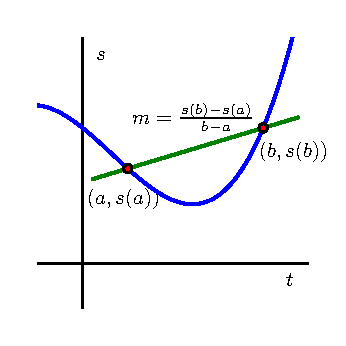
\includegraphics{figures/1_1_Summary.eps}
%\caption{The graph of position function $s$ together with the line through $(a,s(a))$ and $(b,s(b))$ whose slope is $m = \frac{s(b)-s(a)}{b-a}$.  The line's slope is the average rate of change of $s$ on the interval $[a,b]$.} \label{F:1.1.Summary}
%\end{center}
%\end{figure}

\item Given a moving object whose position at time $t$ is given by a function $s$, the average velocity of the object on the time interval $[a,b]$ is given by $AV_{[a,b]} = \frac{s(b) - s(a)}{b-a}$.  Viewing the interval $[a,b]$ as having the form $[a,a+h]$, we equivalently compute average velocity by the formula $AV_{[a,a+h]} = \frac{s(a+h) - s(a)}{h}$.
\item The instantaneous velocity of a moving object at a fixed time is estimated by considering average velocities on shorter and shorter time intervals that contain the instant of interest.
\end{summary}

\end{document}
%-------------------
% END DOCUMENT
%-------------------